% !TeX spellcheck = en_GB
\documentclass[a4paper,kul]{kulakarticle} %options: kul or kulak (default)

\usepackage[utf8]{inputenc}
\usepackage[english]{babel}
\usepackage[T1]{fontenc}
\date{Academic year 2023 -- 2024}
\address{
        Bachelor of Engineering Technology \\
        Complex Digital Design (B-KUL-T3WDO2)\\
        Balasch Masoliver Josep}
\title{Lab report Complex Digital Design}
\author{Robbe Decapmaker, Kobe Michiels}
\usepackage{hyperref}
\usepackage{graphicx}
\usepackage{amsmath, amssymb, amsthm}
%\usepackage{siunitx} %cdd_report.tex: error: 18: File `siunitx.sty' not found. \usepackage
\usepackage{flafter}
\usepackage{pdfpages}
\usepackage{pgfplots}
\usepackage{caption}
\usepackage{subcaption}
\usepackage{datetime2}
\usepackage{subfiles}
\usepackage{multicol}
\setlength{\columnsep}{1cm}
\newcommand{\Lapl}{\ensuremath{\mathcal{L}}}

\usepackage{titlesec}
\usepackage[shortlabels]{enumitem}

\setcounter{secnumdepth}{4}

\titleformat{\paragraph}
{\normalfont\normalsize\bfseries}{\theparagraph}{1em}{}
\titlespacing*{\paragraph}
{0pt}{3.25ex plus 1ex minus .2ex}{1.5ex plus .2ex}

\hypersetup{
	pdftitle={Lab report Complex Digital Design},
	pdfsubject={},
	pdfauthor={Robbe Decapmaker, Kobe Michiels},
	pdfkeywords={}
}

\begin{document}

\maketitle
\section{Introduction}

\section{Features}

% A summary of the features of your final project. For the mandatory assignment, you should provide the maximum ADDER_WIDTH tolerated by your design and the number of cycles your design requires to complete a 512-bit addition. If you have completed any of the optional assignments, make sure to summarize them as well in this part.

\section{Technical description}

% A technical description of your main arithmetic designs in the final project. For the improved combinational adder, you should explain the strategy you have followed and provide a high-level diagram of the design. The diagram should be similar to the ones seen in the lectures. For the optional features, you should also provide an explanation and, if required for comprehension, a high-level diagram.

The implementation of our 128 bit variable sized carry select adder follows the principles described in Lecture \#3A. We found however, that making a practical implementation of it was more difficult than expected. This is because there are a lot of variables at play which have an influence on the ability of the circuit to get timing closure. To this end, we wrote a python script (\texttt{variable\_generator.py}) which takes in a few settings (defined in \texttt{settings.yml}). This allowed us to make rapid iterations of our structure by tweaking just a few settings:
\begin{description}
	\item[adder.width] The width of the adder (128 bit)
	\item[adder.start\_block] The width of the first ripple carry adder 
	\item[adder.start\_repetition] How many times the width of the first block should be repeated before expanding the subsequent blocks
	\item[adder.max\_block\_width] How wide should a block maximally be to prevent excessive fan-out. 
	\item[adder.block\_size\_increment] How much should we increase the full adder count per block when increasing the block size
\end{description}
These parameters were chosen because we believe they give us good control over the critical path with respect to logic (amount of multiplexers) and propagation (fan-out) delays. \\
\\
In the end we ended up with a configuration as seen in figure \ref{fig:128bit-adder}. The specific performance is detailed in the following sections. 
\begin{figure}[h]
	\centering
	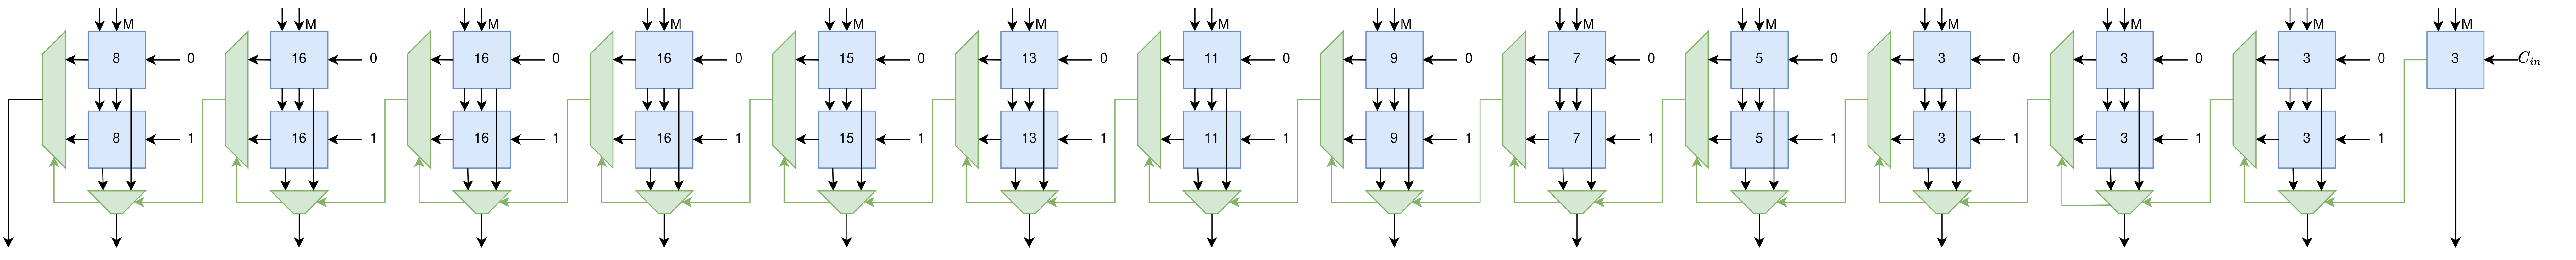
\includegraphics[width=1\linewidth]{images/128bit-ADDER}
	\caption{Schematic of the variable size carry select adder (N=128)}
	\label{fig:128bit-adder}
\end{figure}

\section{Performance evaluation}

% A performance evaluation of your arithmetic designs, including their worst-case delays (as detailed by Vivado in the post-synthesis report) and the area costs (as detailed by Vivado in the post-synthesis utilization report). 

\section{Comparison }

% A comparison of the obtained performance metrics with respect to the original ones from Lab #3, that is, when MP ADDER uses the ripple_carry_adder_Nb with ADDER_WIDTH = 16. Discuss whether the obtained results (speed improvement and area increases) are in line with the expectations.

\section{Conclusion}

\end{document}

